\newpage
\section{Diagrammi di attività}
\subsection{Introduzione}
I diagrammi di attività sono diagrammi che descrivono e modellano un processo. Esso organizza più entità in un insieme di azioni, secondo un determinato flusso.
Il gruppo ha deciso di prendere in esame tre possibili situazioni rilevanti all'interno dell'API Market.

\subsection{Diagramma di attività relativa alla ricerca di una API}
\begin{figure} [H]
	\centering
	\includegraphics[height=0.9\textheight]{"IMG/att_Ricerca_API"}
	\caption{Diagramma di attività che descrive la ricerca di una API}
\end{figure}
\begin{itemize}
	\item \textbf{Precondizioni}: l'utente si trova nella schermata di ricerca API;
	\item \textbf{Postcondizioni}: l'utente ha individuato le API adatte alle sue necessità e, se vuole, potrà effettuare una nuova ricerca oppure visualizzare una delle API risultato;
	\item \textbf{Descrizione}: l'utente riempie un box di ricerca con le keywords desiderate e visualizza la lista delle API corrispondenti alle keywords. All'utente si presentano due possibili scelte: effettuare una nuova ricerca con keywords diverse, se i risultati della ricerca non soddisfano le sue aspettative, oppure visualizzare la pagina dedicata ad una delle API risultato. Nella schermata di visualizzazione di una API si presentano due possibili scenari: dopo aver consultato la pagina dell'API, se l'utente è soddisfatto può decidere di proseguire l'acquisto, situazione descritta nel diagramma \textit{"Acquisto API"}, oppure ritornare ai risultati della ricerca precedente (da cui potrà anche effettuare una nuova ricerca).
\end{itemize}

\newpage
\subsection{Diagramma di attività relativa all'acquisto di una API}
\begin{figure}[h]
	\centering
	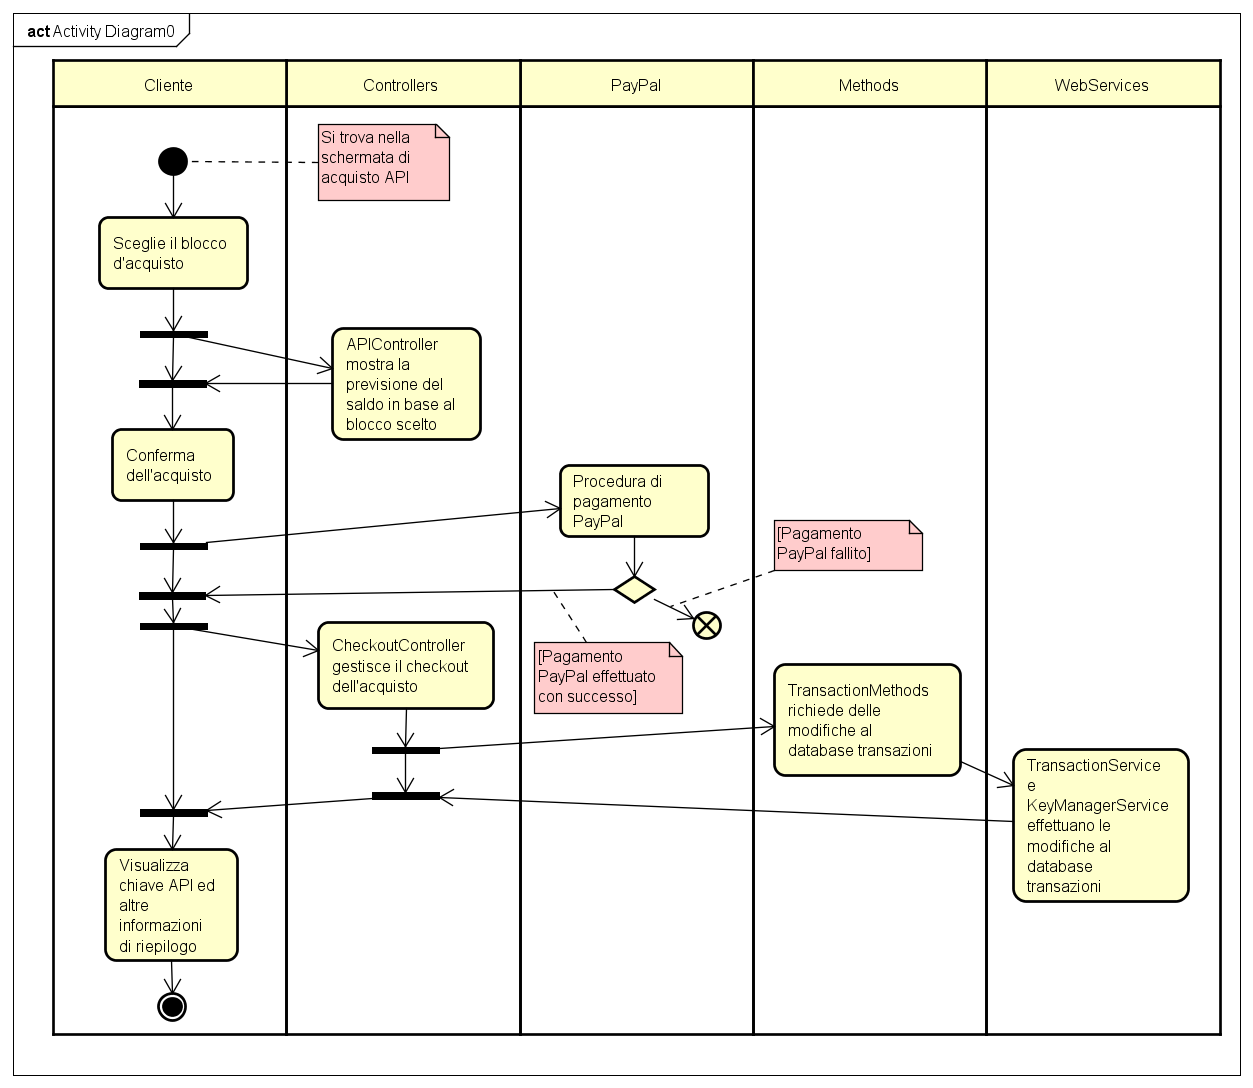
\includegraphics[width=1.0\linewidth]{IMG/att_Acquisto_API}
	\caption{Diagramma di attività che descrive l'acquisto di una API}
	\label{fig:acquistoapi}
\end{figure}

\begin{itemize}
	\item \textbf{Precondizioni}: l'utente si trova nella schermata di acquisto di una API;
	\item \textbf{Postcondizioni}: l'utente ha acquistato una API e ne ha visualizzato la chiave API;
	\item \textbf{Descrizione}: l'utente visualizza le informazioni d'acquisto dell'API desiderata, può scegliere il blocco d'acquisto preferito e visualizzare la previsione del saldo. Se il cliente confermerà l'acquisto, verrà reindirizzato alla procedura PayPal per il pagamento. In caso di insuccesso, l'acquisto verrà annullato. In caso di successo, API Market genererà la chiave API ed aggiungerà la transazione al rispettivo database; poi mostrerà all'utente la chiave API generata assieme ad altre informazioni di riepilogo, terminando la procedura di acquisto.
\end{itemize}

\newpage
\subsection{Diagramma di attività relativa all'inserimento di una API}
\begin{figure}[h]
	\centering
	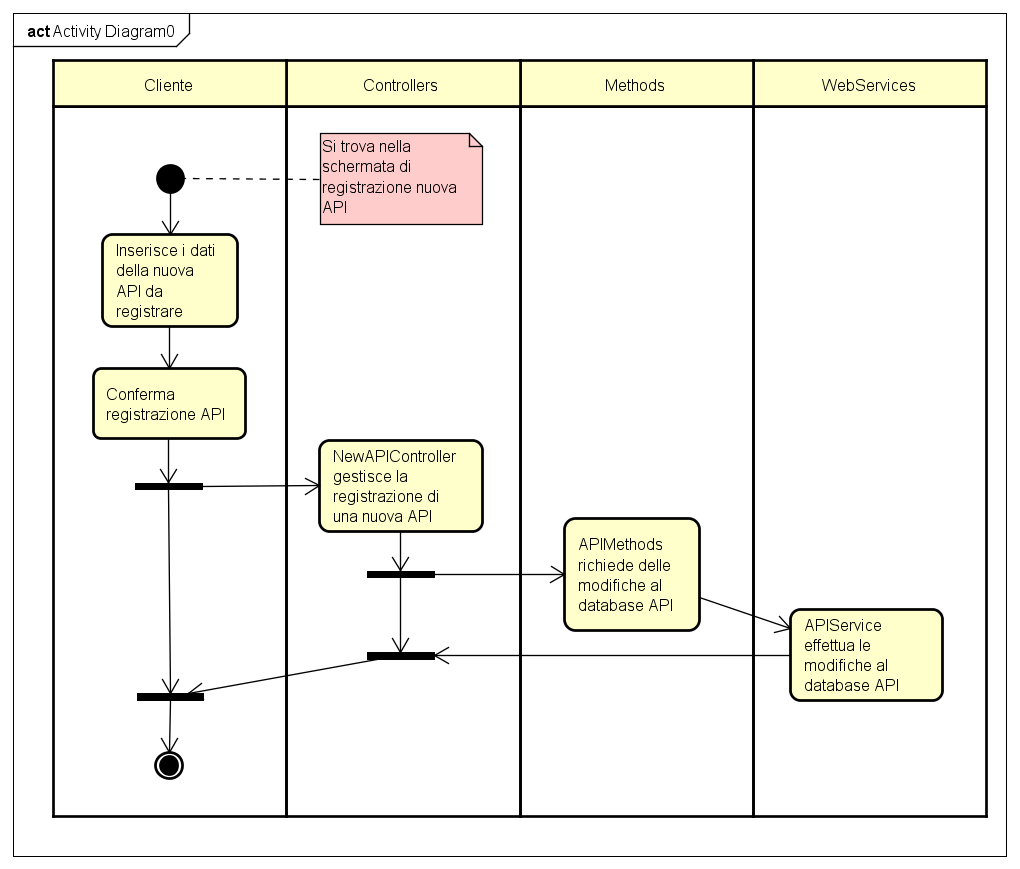
\includegraphics[width=1.0\linewidth]{IMG/att_Registrazione_API}
	\caption{Diagramma di attività che descrive la registrazione di una nuova API}
	\label{fig:inserimentoapi}
\end{figure}


\begin{itemize}
	\item \textbf{Precondizioni}: l'utente si trova nella schermata di registrazione di una nuova API;
	\item \textbf{Postcondizioni}: l'utente ha registrato una nuova API in API Market;
	\item \textbf{Descrizione}: l'utente inserisce i dati richiesti per la registrazione della nuova API. I dati in questione sono elencati di seguito:
	\begin{itemize}
		\item Nome dell'API;
		\item Categoria di appartenenza dell'API;
		\item Codice dell'interfaccia dell'API;
		\item Documentazione dell'API;
		\item Policy di vendita dell'API, ovvero:
		\begin{itemize}
			\item \textbf{Policy a chiamate}: calcolata in euro per ogni chiamata da parte di un acquirente dell'API;
			\item \textbf{Policy a traffico}: calcolata in euro per ogni kB trasmesso ad un acquirente dell'API;
			\item \textbf{Policy a tempo}: calcolata in euro per ogni minuto di elaborazione da parte di un acquirente dell'API.
		\end{itemize}
		\item Guadagno netto dell'API in base alla policy scelta;
		\item Logo dell'API;
		\item Indirizzo dell'API;
				
	\end{itemize}
	Successivamente può confermare la registrazione dell'API, che verrà salvata in API Market e resa disponibile a tutti gli utenti.
\end{itemize}
